\documentclass[tikz, border=5pt]{standalone}
\usepackage{tikz}
\usepackage{amsmath}

\begin{document}
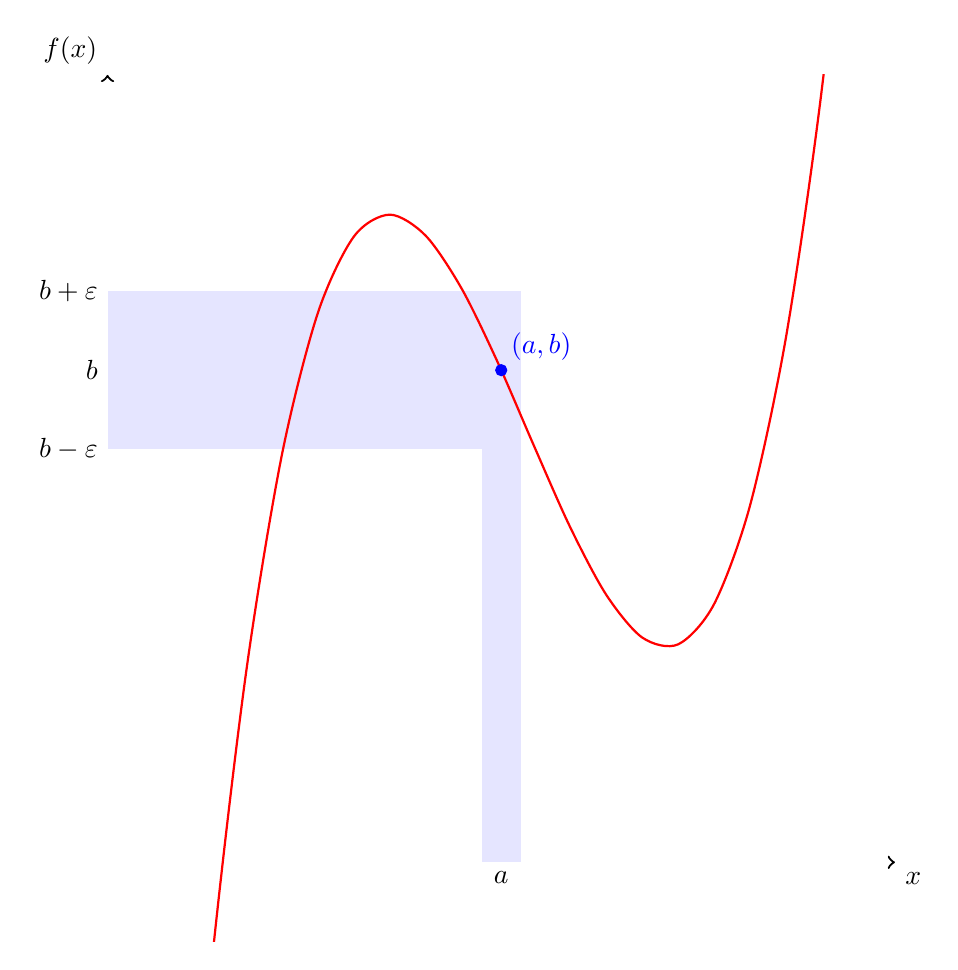
\begin{tikzpicture}[scale=2]
    %% Epsilon-delta

    % Parameters
    \def\xmax{5}
    \def\ymax{5}
    \def\a{2.5}
    \def\f#1{(#1 - 3)^3 + (#1 - 4)^2 + 1}
    \def\eps{0.5}

    \def\xmin{-0.5}
    \def\ymin{-0.5}

    % Compute f(a)
    \pgfmathsetmacro\b{\f{\a}}

    % Compute suitable delta
    \def\del{0.5}
    \pgfmathsetmacro{\fplus}{abs(\f{\a+\del} - \b)}
    \pgfmathsetmacro{\fminus}{abs(\f{\a-\del} - \b)}
    \pgfmathsetmacro{\maxdiff}{max(\fplus,\fminus)}
    % Reduce delta if maxdiff > eps
    \pgfmathsetmacro{\newdel}{\del}
    \pgfmathsetmacro{\maxiter}{20}
    \pgfmathsetmacro{\iter}{0}
    \loop
    \ifdim \maxdiff pt > \eps pt
    \pgfmathsetmacro{\newdel}{\newdel/2}
    \pgfmathsetmacro{\fplus}{abs(\f{\a+\newdel} - \b)}
    \pgfmathsetmacro{\fminus}{abs(\f{\a-\newdel} - \b)}
    \pgfmathsetmacro{\maxdiff}{max(\fplus,\fminus)}
    \pgfmathsetmacro{\iter}{\iter+1}
    \repeat
    % Final delta
    \def\del{\newdel}

    % Plot axes
    \draw[thick,->]
    -- (\xmin,0)
    -- (\xmax,0)
    node[anchor=north west] {\( x \)};

    \draw[thick,->]
    -- (0,\ymin)
    -- (0,\ymax)
    node[anchor=south east] {\( f(x) \)};

    % Shade epsilon band
    \fill[blue,opacity=0.1]
    -- (0,{\b-\eps}) rectangle ({\a+\del},{\b+\eps});

    % Shade delta band
    \fill[blue,opacity=0.1]
    -- ({\a-\del},0) rectangle ({\a+\del},{\b-\eps});

    % Boxes
    \draw[dashed]
    -- (0,\b)
    -- (\a,\b)
    -- (\a,0);

    \draw[dashed]
    -- (0,{\b+\eps})
    -- ({\a+\del},{\b+\eps})
    -- ({\a+\del},0);

    \draw[dashed]
    -- (0,{\b-\eps})
    -- ({\a-\del},{\b-\eps})
    -- ({\a-\del},0);

    % Plot function
    \clip (\xmin,\ymin) rectangle (\xmax,\ymax);
    \draw[thick,red,domain=\xmin:\xmax,smooth,variable=\x]
    plot ({\x},{\f{\x}});

    % Labels
    \filldraw[blue]
    -- (\a,\b)
    circle (1pt)
    node[anchor=south west] {\( (a, b) \)};

    \node at (0,\b) [anchor=east] {\( b \)};
    \node at (\a,0) [anchor=north] {\( a \)};

    \node at (0,{\b+\eps}) [anchor=east] {\( b + \varepsilon \)};
    \node at (0,{\b-\eps}) [anchor=east] {\( b - \varepsilon \)};

\end{tikzpicture}
\end{document}
